\section{Evaluation}
\label{sec:eval}

We evaluate \tool{} on real serverless workflows: RQ1, does it detect the defect classes of
Figure~\ref{fig:intro}? RQ2, what does verification cost? RQ3, does the shared-IR design extend
beyond AWS? Controlled mutation studies measure per-check detection power; unmodified workflows,
deployment templates, issue reports, and fixed-bug pairs provide real-world evidence.

\subsection{Setup and corpus}
\label{sec:eval:corpus}

We organize evidence by realism before size. The foreground set is public but deployment-shaped:
six industrial-topology \texttt{aws-samples} workflows, including AWS Serverless Airline Booking
\texttt{ProcessBooking}, a canonical serverless benchmark~\cite{awsServerlessAirline,eismann2022stability};
\textbf{55} \texttt{serverless-patterns} workflows read from SAM/CloudFormation deployments; and
\textbf{24} AWS Solutions Library artifacts (\textbf{26} machines), including CDK-synthesized
enterprise orchestrators. These public artifacts are reproducible stand-ins for proprietary
industrial definitions, not arbitrary toy repositories. Broader strata provide coverage and stress:
\textbf{193} AWS sample workflows, \textbf{66} CNCF examples, and \textbf{95} independent ASL
definitions.

The 193-workflow AWS stratum is mined exhaustively from every parseable \asl{} definition while
excluding build-configuration JSON. It contains 1{,}355 state entries: 1{,}354 valid states (median
6, max 33) plus one malformed non-state \texttt{QueryLanguage} entry reported as \code{SC0010}. It
has 166 \texttt{Choice}, 64 \texttt{Map}, and 33 \texttt{Parallel} states; 84 workflows with retries;
and 51 with catch handlers. It also includes \textbf{5} JSONata-mode, \textbf{19} Distributed Map,
and \textbf{18} nested-\texttt{states:startExecution} workflows across nine AWS services. All
experiments use a Rust~1.96 release build on a commodity laptop.

\subsection{Detection in the wild}
\label{sec:eval:wild}

Run over the corpus with optional inference enabled as a non-blocking adoption mode, \tool{} flags
\textbf{99 of 193} workflows. The native findings are small but concrete. Nine
workflows have a \texttt{Choice} with no \texttt{Default} (\code{SC0007}), a runtime-risk warning
because an input matching no rule fails. One workflow nests a machine-level \texttt{QueryLanguage}
directive inside \texttt{States} (\code{SC0010}). Another 33 callback tasks lack a timeout or
heartbeat (\code{SC6001}); each can wait up to the platform limit while holding business state open.
The sound \code{SC1101}, dead-guard \code{SC1110}, and
concurrency checks are silent on the default corpus run; their power is exercised below.

The semantic warnings surface adoption targets: \code{SC3001}: 36, \code{SC4001}: 117, and
\code{SC4010}: 28. These are an \emph{advisory} adoption aid, not a verification claim---the paper's
evidentiary weight is on the label-free sound native tier (\code{SC1101}, Theorem~\ref{thm:soundness})
and the declared tier. To evaluate them without leakage, we \emph{freeze} the inference rules (pinned
by their source blob hash), and split the human-labelled gold (23 workflows, double-labelled by two
annotators) into a \textbf{design} partition of 10 workflows that informed rule authoring and a
\textbf{hold-out} of 13 labelled afterward. On the hold-out, per-check inter-annotator agreement is
high ($\kappa\,{=}\,0.97$ idempotency, $0.98$ persistence) and warning precision is \textbf{27/29
(93\%)} for \code{SC4001}, \textbf{3/3} for \code{SC3001}, and \textbf{4/4} for \code{SC4010}; the
underlying property inference is high-recall but moderate-precision (idempotency recall $0.94$,
precision $0.56$; false-omission rate $0.06$), exactly the profile of an adoption aid that prefers to
surface a risk over hiding one. The downstream declared check \code{SC4011} is silent on the wild
corpus because no workflow declares a compensator. The declared Saga fixtures contain 7 persistent
steps; \tool{} accepts the complete compensation chains and, on the injected chain-break case, reports
exactly \texttt{CreateOrder} and \texttt{ReserveInventory}, the upstream effects that would leak.

\subsection{Detection power versus existing validators}
\label{sec:eval:mut}
\label{sec:eval:baseline}

For each applicable workflow, \texttt{stepcheck mutate} injects one defect and re-verification
counts a detection only when the expected diagnostic increases over the unmutated baseline. Across
\textbf{616} mutants in six corpus-scale classes, \tool{} detects every injected defect
(Figure~\ref{fig:detection}a and Table~\ref{tab:baseline}). This is per-check reliability on
targeted operators, not a claim of complete bug coverage.

We compare against the validators developers already use---\texttt{statelint},
\texttt{asl-validator}, and AWS's authoritative \texttt{ValidateStateMachineDefinition}. This is a
complementarity test, not a superiority claim: those validators catch schema-expressible dangling
transitions and broken JSONPath syntax, but do not attempt unsafe retries, missing compensations,
races, or heartbeat/timeout violations. In the wild the two flag largely disjoint workflows
(Figure~\ref{fig:detection}b): \tool{} alone flags 36, the panel alone 55, mostly schema nits.

\begin{figure}[t]
\centering
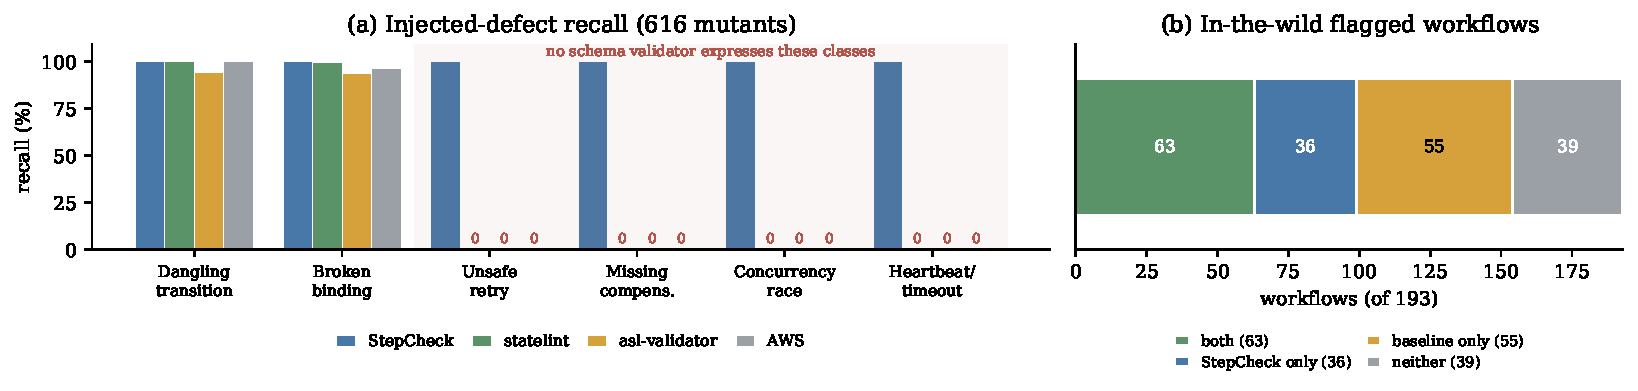
\includegraphics[width=0.92\textwidth]{figures/eval-detection.pdf}
\caption{Detection versus the validator panel: (a) recall over 616 mutants---\tool{} detects all
six classes, existing validators none of the four semantic ones; (b) mostly disjoint in-the-wild
coverage over the 193 workflows.}
\label{fig:detection}
\end{figure}

\begin{table}[t]
\centering\small
\caption{Injected-defect detection over 616 mutants. A mutant counts as detected only when a tool
emits a new problem naming the injected fault; incidental schema nits are not credited.}
\label{tab:baseline}
\setlength{\tabcolsep}{4pt}
\resizebox{\textwidth}{!}{%
\begin{tabular}{@{}llrrrrr@{}}
\toprule
 & & & & \multicolumn{3}{c@{}}{Baseline validators} \\
\cmidrule(l){5-7}
Defect class & Check & Appl. & \tool{} & \texttt{statelint} & \texttt{asl-val.} & AWS \\
\midrule
Dangling transition & \code{SC0002} & 166 & 166 (100\%) & 166 (100\%) & 156 (94\%) & 166 (100\%) \\
Broken data binding & \code{SC1003} & 141 & 141 (100\%) & 140 (99\%) & 132 (94\%) & 136 (96\%) \\
Unsafe retry & \code{SC3001} & 103 & 103 (100\%) & \textbf{0} & \textbf{0} & \textbf{0} \\
Missing compensation & \code{SC4001} & 19 & 19 (100\%) & \textbf{0} & \textbf{0} & \textbf{0} \\
Concurrency interference & \code{SC5001} & 21 & 21 (100\%) & \textbf{0} & \textbf{0} & \textbf{0} \\
Temporal heartbeat/timeout & \code{SC6003} & 166 & 166 (100\%) & \textbf{0} & \textbf{0} & \textbf{0} \\
\midrule
\textbf{Total} & & \textbf{616} & \textbf{616 (100\%)} & \textbf{306 (50\%)} & \textbf{288 (47\%)} & \textbf{302 (49\%)} \\
\bottomrule
\end{tabular}}
\end{table}

\subsection{Comparison with three formal workflow verifiers}
\label{sec:eval:bprove}

Schema validators are the tools a developer reaches for, but they are not a research-grade adversary.
We therefore also compare against \emph{three} formal workflow-soundness verifiers, run locally:
\textbf{Woflan}~\cite{woflan}, the classical workflow-net soundness verifier of van der Aalst and
Verbeek (via \texttt{pm4py}); \textbf{BPMN Analyzer 2.0}~\cite{bpmnanalyzer}, a recent BPMN-specific
model checker of Kr\"auter et al. (a Rust reachability-graph checker with counterexamples); and
\textbf{BProVe}~\cite{bprove}, via its BPMNOS BPMN parser plus Maude model checker. The baselines
decide the standard workflow-soundness subproperties---\emph{safeness}, \emph{option to complete},
\emph{proper completion}, and, where exposed, \emph{no dead activities}. We
encode each \asl{} workflow into a BPMN workflow net (rules A--E: Choice $\to$ exclusive gateway,
Parallel $\to$ parallel split/join, Map $\to$ activity, Catch $\to$ error gateway, terminals merged to
one end event), and run the same confound-free protocol: \texttt{emit} control versus \texttt{mutate}
mutant, crediting a verifier only when the mutant encoding carries a fresh soundness violation.

The result is \emph{complementarity, not superiority} (Table~\ref{tab:woflan}). On the one
control-flow class all can express, dangling transitions (\code{SC0002}), the verifiers detect fresh
violations at different recall levels: Woflan $95\%$, BPMN Analyzer $87\%$, and BProVe $69\%$. On the
classes that are not workflow-net soundness properties---data binding, unsafe retry, and
heartbeat/timeout---all are silent by construction while \tool{} detects all; \code{SC1101} data-flow
has no BPMN expression at all. Compensation and concurrency appear only as structural side effects
for some baselines (Woflan/BPMN Analyzer $7/19$ compensation; BProVe $2/19$ compensation and $1/21$
concurrency). Crucially, the baselines over-report on valid AWS serverless workflows: Woflan and BPMN
Analyzer each flag \textbf{16 of 193} ($8.3\%$), and BProVe flags \textbf{56 of 193} ($29\%$), because
independent, multi-terminal branch structure is not always a well-handled workflow net---a semantic
mismatch between classical soundness and \asl{}, not a \tool{} finding. Confidence intervals are exact
(Clopper--Pearson); no recall is a bare ``100\%'', and even on the small semantic classes Fisher exact
separates \tool{} from each verifier at $p<4\times10^{-5}$.

BProVe's soundness checking addresses BPMN soundness and incidental structural effects, while
\tool{}'s ASL-native data-flow covers \code{SC1101}; thus \code{SC1101} is StepCheck versus
out-of-scope, not a BProVe miss. Likewise, \code{SC6003} is a native \asl{} temporal bound, not a BPMN
dead-activity property.

\begin{table}[t]
\centering\small
\setlength{\tabcolsep}{3pt}
\caption{\tool{} versus three formal verifiers (Woflan; BPMN Analyzer 2.0; BProVe) over 193 workflows,
per-class recall with exact 95\% CIs. The tools are complementary: all overlap on \code{SC0002};
\tool{} is unique on the data-flow / atomicity / concurrency / temporal classes with no workflow-net
expression.}
\label{tab:woflan}
\resizebox{\textwidth}{!}{%
\begin{tabular}{@{}llrllll@{}}
\toprule
Defect class & Check & $n$ & \tool{} (CI) & Woflan & BPMN-Anlz. & BProVe \\
\midrule
Dangling transition & \code{SC0002} & 166 & 1.00 [.98,1] & 0.95 & 0.87 & 0.69 \\
Broken data binding & \code{SC1003} & 141 & 1.00 [.97,1] & 0.00 & 0.00 & 0.00 \\
Unsafe retry & \code{SC3001} & 103 & 1.00 [.97,1] & 0.00 & 0.00 & 0.00 \\
Missing compensation & \code{SC4001} & 19 & 1.00 [.82,1] & 0.37 & 0.37 & 0.11 \\
Concurrency interference & \code{SC5001} & 21 & 1.00 [.84,1] & 0.00 & 0.00 & 0.05 \\
Temporal heartbeat/timeout & \code{SC6003} & 166 & 1.00 [.98,1] & 0.00 & 0.00 & 0.00 \\
\midrule
\multicolumn{3}{@{}l}{Formal-verifier over-report on \emph{valid} wf.} & & 16/193 (8.3\%) & 16/193 (8.3\%) & 56/193 (29\%) \\
\bottomrule
\end{tabular}
}
\end{table}

Because Figure~\ref{fig:intro} uses AWS Serverless Airline Booking (SAB), we also run the same
three-verifier protocol on \texttt{ProcessBooking} alone (Table~\ref{tab:sab}). The clean SAB
workflow is accepted by Woflan, BPMN Analyzer, and BProVe. On applicable SAB mutants, all tools catch
the purely structural dangling transition, but only \tool{} catches the ASL-native binding, retry,
compensation, and temporal defects; SAB has no applicable concurrency-interference site. This is not
a statistical claim, but a benchmark-specific witness that the complementarity in Table~\ref{tab:woflan}
holds on the paper's canonical industrial proxy.

\begin{table}[t]
\centering\small
\setlength{\tabcolsep}{4pt}
\caption{SAB \texttt{ProcessBooking}: per-class detection on one applicable mutant per class.}
\label{tab:sab}
\begin{tabular}{@{}llcccc@{}}
\toprule
Defect class & Check & \tool{} & Woflan & BPMN-Anlz. & BProVe \\
\midrule
Dangling transition & \code{SC0002} & Yes & Yes & Yes & Yes \\
Broken data binding & \code{SC1003} & Yes & No & No & No \\
Unsafe retry & \code{SC3001} & Yes & No & No & No \\
Missing compensation & \code{SC4001} & Yes & No & No & No \\
Concurrency interference & \code{SC5001} & n/a & n/a & n/a & n/a \\
Temporal bound & \code{SC6003} & Yes & No & No & No \\
\bottomrule
\end{tabular}
\end{table}

\paragraph{The quantitative axis is orthogonal.}
Both baselines above check \emph{control-flow soundness}. A different, quantitative line of work
verifies workflow \emph{performance}: Su and Liu~\cite{suliu2024} model AWS Step Functions as
semi-Markov chains and compute first-passage-time (FPT) moments---up to the fourth moment for a
$10{,}000$-state model in ${\approx}70$\,s---to profile execution-time distributions. This is
\emph{complementary and orthogonal} to \tool{}: our temporal checks are static, single-mode
$\tau$-bounds (\code{SC6001}/\code{SC6003}: is a callback bounded, is a heartbeat consistent with its
timeout), whereas Su and Liu's are probabilistic multi-order FPT moments over a stochastic model.
\tool{} targets temporal \emph{correctness} at build time, not SLA \emph{prediction}; the two answer
different questions and could compose (a static gate feeding a quantitative model).

\subsection{Industrial case study and build-time gate}
\label{sec:eval:industrial}

We assemble an industrial-topology set of six workflows: four \texttt{aws-samples}
production patterns (a travel-reservation saga with retry on every forward task and a three-step
compensation chain, a CDK saga, an inventory reserve-stock saga, and a checkout workflow), a Map-based
ETL aggregator, and the AWS Serverless Airline Booking \texttt{ProcessBooking} saga
(12 states: reserve flight/booking\,$\to$\,collect-payment\,$\to$\,confirm\,$\to$\,notify, with
release-seat / cancel-booking / refund-payment compensation and a booking DLQ), read \emph{directly}
from the SAM \texttt{template.yaml} in the project's \texttt{master} branch by the CloudFormation
front end---\texttt{stepcheck check src/backend/booking/template.yaml} needs no manual extraction.
On these sagas \tool{} surfaces advisory retry-safety and compensation-coverage findings
(\code{SC3001}/\code{SC4001}) on durable steps, while Woflan reports all six sound. The same
fair-class protocol reproduces the complementarity of Table~\ref{tab:woflan} (\tool{} $100\%$ per
class; Woflan only \code{SC0002}).

As a build-time gate, \texttt{stepcheck check -{}-deny-warnings} runs at CI cost. We inject
$0/1/5$ defects at build time and report, per level, the gate's build-fail catch-rate, the platform
validator's silent pass-through (\texttt{asl-validator}, the schema check AWS's
\texttt{ValidateStateMachineDefinition} performs---does the mutant still ``validate'' and deploy?),
and the gate latency (Table~\ref{tab:gate}). The practitioner-facing result: at a single injected
\emph{semantic} defect the gate fails the build on \textbf{every} workflow while the platform accepts
\textbf{$80\%$} of them (the defect would deploy); at five defects the gate still catches all, and
the platform only rejects the ones with a co-injected \emph{syntactic} fault while silently passing
the semantic ones. Gate latency is stable in the defect count---p95 $16$--$21$\,ms end-to-end
including process start---so the gate is a genuine drop-in (configuration in the artifact).

\begin{table}[t]
\centering\small
\setlength{\tabcolsep}{5pt}
\caption{Build-time gate on the industrial set: with $M$ defects injected, StepCheck's build-fail
catch-rate vs. the platform validator's silent pass-through (accepts $\Rightarrow$ would deploy), and
gate latency. The gate catches what the platform deploys, at CI cost.}
\label{tab:gate}
\resizebox{\textwidth}{!}{%
\begin{tabular}{@{}rlll@{}}
\toprule
Injected defects & \tool{} gate catch & Platform silent-pass & Gate p50/p95/p99 (ms) \\
\midrule
0 (clean) & --- & $0.83$ & $12.5/15.9/28.0$ \\
1 (semantic) & $\mathbf{1.00}$ & $0.80$ & $11.8/17.1/29.5$ \\
5 (mixed) & $\mathbf{1.00}$ & $0.00$ & $13.0/21.4/26.6$ \\
\bottomrule
\end{tabular}
}
\end{table}

\subsection{Data-flow provenance: soundness, power, and reach}
\label{sec:eval:dataflow}

The central \code{SC1101} claim is no false positives. In the default native corpus run it fires zero
times. To exercise its power, the typed-tier mutator is seeded with declared input fields and injects
a missing-field read into each of the \textbf{126} workflows with a suitable site. With service/output
shape modeling enabled (\texttt{--result-shapes}), \tool{} detects \textbf{88 of 126 (70\%)}. An
independent certificate pass then discharges the emitted reports from a finite widened-fixpoint
invariant: across \textbf{207} analyzed machines it checks \textbf{1{,}146} normal/catch postcondition
obligations, certifies all \textbf{88} emitted \code{SC1101} reports, and finds zero failed
obligations or diagnostic mismatches. A separate concrete execution oracle remains as a
code-disjoint empirical check: on the same configured population it reports zero present-field
counterexamples on bounded loop-unrolled reaching paths.

The check is not vacuous: it catches the \texttt{amount}/\texttt{total} miss validators accept, and
flow-sensitive misses through \texttt{ResultPath} merges that adjacent-task field-subset checks miss.
The implementation resolves dotted and quoted-bracket member paths; \texttt{--result-shapes} treats
declared task-output schemas as closed-world result records and adds closed top-level envelopes for
common AWS integrations (Lambda invoke, DynamoDB, SNS, SQS, EventBridge, and Step Functions child
execution). The remaining misses are behind unsupported or templated service results, arrays, or
complex selectors that still lift to $\top$.

The modeled fragment covers most real reads: of the corpus's genuine document-field references,
\textbf{92\%} use dotted access and resolve precisely, and \textbf{8\%} use bracket/wildcard/filter
syntax abstracted to $\top$ (\texttt{\$\$} context and \texttt{States.*} operands are not document
references; \texttt{stepcheck path-coverage}, full breakdown in the technical report).

\subsection{Real defects in the wild}
\label{sec:eval:realbugs}

We mined fix-commit pairs whose diff edits an \asl{} definition and ran \tool{} on both revisions.
In \textbf{7 of 39} pairs a finding is present only on the buggy revision; adjudication confirms
\textbf{6} genuine defects across five repositories, one an official AWS sample
(Table~\ref{tab:realbugs}); four are semantic/logic classes no schema validator expresses. This is
existence evidence, not a prevalence estimate.

Beyond fix-commit diffs, we also searched issue trackers for user-reported defects: closed
GitHub issues whose quoted runtime error is exactly the fault \tool{}'s sound tier prevents. Three are
textbook \code{SC1101}, one in an \emph{official AWS workshop}: \emph{serverless-coffee-workshop} \#56
(``The JSONPath \texttt{\$.detail.orderId} \ldots could not be found in the input
\texttt{\{\allowbreak"orderNumber":"10"\}}'', filed by a user who reran the lab three times),
\emph{campus-compute} \#32 (an audit step reads a job field wiped by a preceding SNS \texttt{Publish}
whose default \texttt{ResultPath} overwrites the document), and \emph{turbofan} \#1 (a fan-out reads
\texttt{\$.input}, absent from the trigger payload). These machines are built in CDK, but CDK
synthesizes \asl{}: for \#32 we checked out the buggy commit, ran \texttt{cdk synth}, and extracted
the \emph{real} 14-state definition---on which \tool{} flags exactly \code{SC1101} at
\texttt{AuditLogFailed} reading \texttt{\$.execution\_id}, the reported fault. The others are confirmed
on a minimal reproduction of the reported structure with the issue URL and verbatim error recorded.
These are user-filed defects, not author-selected diffs, and \code{SC1101} is the most
issue-tracker-visible class because it fails with an explicit JSONPath error. A second pass over
standalone \asl{} files from independent repositories surfaces a real \code{SC3001} in
\emph{solo-vault-backend}'s pipeline (an SQS send, non-idempotent, retried on \texttt{TaskFailed}); a
\emph{data-meshy} subscription saga has proper compensation and produces no finding.

\begin{table}[t]
\centering\small
\setlength{\tabcolsep}{4pt}
\renewcommand{\arraystretch}{1.15}
\caption{Confirmed in-the-wild defects re-discovered on deployed artifacts.}
\label{tab:realbugs}
\begin{tabular}{@{}lp{3.1cm}p{5.9cm}@{}}
\toprule
\textbf{Code} & \textbf{Repository} & \textbf{Defect fixed} \\
\midrule
\code{SC1101} & aws-batch-runtime-monitoring & document field used instead of context input \\
\code{SC1101} & serverless-ai-fitness & tasks read fields never produced \\
\code{SC1110} & serverless-ai-fitness & subscriber branch unreachable \\
\code{SC6001} & leave-management & callback can hang indefinitely \\
\code{SC0002} & airway-shipment-orchestrator & transition targets missing state \\
\code{SC0003/4/5} & video-translation & string \texttt{End} leaves dead states \\
\bottomrule
\end{tabular}
\end{table}

\subsection{Cost, overhead, and deployment}
\label{sec:eval:cost}
\label{sec:eval:roundtrip}

Verification is cheap: the eight passes average $\approx$\textbf{39}\,$\mu$s per workflow (median
$\approx$25\,$\mu$s, max $\approx$1.1\,ms), and the check adds no runtime component because it runs
before deployment. This corpus is not only acyclic examples: it contains \textbf{84} workflows with
\texttt{Retry}, \textbf{52} with \texttt{Map}, \textbf{29} with \texttt{Parallel}, \textbf{55} with
control-flow cycles, and nesting depth up to three. To check cost on production-shaped artifacts, we
also timed the real industrial set (6 workflows, 65 recursive states, retries/catches plus
\texttt{Parallel} and \texttt{Map} topologies): mean $\approx$\textbf{91}\,$\mu$s per workflow, median
$\approx$100\,$\mu$s, max $\approx$0.17\,ms, total $\approx$0.55\,ms. Across the AWS Solutions corpus
(24 workflows/artifacts, 385 recursive states), mean cost is $\approx$\textbf{0.28}\,ms per workflow
(median $\approx$0.12\,ms, max $\approx$1.58\,ms, total $\approx$6.70\,ms). The CDK-synthesized AWS
Solutions subset used for gate timing includes 173 recursive states, five \texttt{Map}-bearing
templates, four cyclic workflows, and one nested-\texttt{Map} template (depth two); running the checker
as a CI process on these templates costs p50/p95 $\approx$15.7/20.9\,ms, while the smaller industrial
set costs $\approx$9.4/11.3\,ms. Synthetic chains and stress shapes remain scalability sanity checks:
30{,}000 acyclic states verify in $\approx$0.13\,s, a 512-branch \texttt{Parallel} fan-out
(2{,}051 states) in $\approx$49\,ms, and a 160-level nested \texttt{Map} in $\approx$11\,ms.

The DSL stays concise (20 declarations expand to a 119-line annotated \asl{} definition). Our live
deployment check spans three real AWS execution models, each deploying a StepCheck-verified
definition unmodified (only \texttt{FunctionName} rebound to a stand-in Lambda) to
\texttt{SUCCEEDED}: the order workflow as a synchronous \emph{Express} machine; the same definition
as an asynchronous \emph{Standard} machine, whose durable history retains all \textbf{24} events
(Express retains none); and a DSL-verified order variant with a bounded \code{.waitForTaskToken}
approval gate---which Express cannot run---deployed as Standard, where the run \emph{pauses} at the
callback and an external \texttt{SendTaskSuccess} resumes it to completion (\textbf{30} events). The
deployed callback draws no \code{SC6001} because its \texttt{TimeoutSeconds} bounds the wait; removing
that bound makes the temporal pass flag it pre-deployment. The verified artifact also runs at scale:
across \textbf{100} executions in each non-callback mode it completes \textbf{100/100} times---Express
at p50/p95 $\approx$\textbf{72}/130\,ms and Standard (durable, five state transitions per run) at
p50/p95 $\approx$\textbf{345}/456\,ms of execution time. This is a completion check across execution
models, not a cross-mode performance benchmark. Scripts, per-run timings, and captured runtime logs
ship with the artifact, together with a self-testing GitHub Actions gate
(\texttt{.github/workflows/gate.yml}) that runs the blocking check on every push and asserts, via a
negative test, that an injected defect fails the build. The emitter that makes the DSL-first story deployable is
measured on the full 193-workflow \asl{} corpus: round-tripping through the IR
($\asl\to$IR$\to\asl$) preserves $100\%$ of states and all measured I/O-processing fields
(including \texttt{InputPath}, \texttt{OutputPath}, \texttt{ResultPath}, \texttt{ResultSelector},
\texttt{Parameters}, \texttt{Result}, JSONata \texttt{Arguments}/\texttt{Assign}/\texttt{Output}, and
Map item-selection fields), achieves exact \asl{}-object equality for $99.5\%$ of workflows, and
keeps \texttt{emit} idempotent on all 193. The single non-exact case is a malformed corpus entry with
a non-state marker inside \texttt{States}, which the parser normalizes away rather than re-emitting.

\subsection{Cross-format generalization: CNCF Serverless Workflow}
\label{sec:eval:cncf}

The CNCF front end parses \textbf{66} Serverless Workflow examples and lowers them to the same IR.
Structural, typestate, retry, compensation, concurrency, and temporal checks apply unchanged. Pure
\texttt{jq} field references (\texttt{.a.b}, \texttt{\$\{ .a.b \}}) lower to the same JSONPath read by
the sound \code{SC1101}/\code{SC1110} checks, so field-provenance analysis fires at CNCF
declared-record boundaries---a jq read of a field absent from a task's declared input schema is
flagged. A comparison or presence guard over a document field (\texttt{.a.b == v}, \texttt{.a.b < v},
\texttt{.a.b != null}, and the leading operand of a short-circuiting \texttt{and}/\texttt{or}) likewise
lowers to that field's read, while the remaining composite jq (pipes, arithmetic, object construction,
and \texttt{\$context}/\texttt{\$workflow} runtime references) soundly projects to $\top$. Of
the 66 workflows, \textbf{12} contain such modelable references (18 reference sites); the rest are
schema-free and stay conservative. Mutation detects every injected control-flow defect with a site
(retry 4/4, structural 9/9, concurrency 1/1, temporal 50/50), and where CNCF declares JSON Schemas
\code{SC1010} uses them exactly: a reordered schema-annotated order workflow is rejected with three
contract errors.

\subsection{External validity: independent repositories}
\label{sec:eval:wildext}

To test whether the analyses overfit AWS's own samples, we ran \tool{} on \textbf{95}
further ASL definitions from \textbf{16} public repositories outside the AWS sample collections
(50 domain workflows across 13 repositories, the rest validator fixtures; script and manifest in the
artifact). The sound \code{SC1101} fires on a credit-card transaction-reversal workflow: its
\texttt{Pass} state reconstructs the document through \texttt{Parameters} into a closed record that
drops the \texttt{ledgerEntries} field a downstream \texttt{Map} iterates. This is a flow-sensitive
miss no adjacent-field check sees. The concurrency check flags an IoT firmware-upgrade workflow
whose three \texttt{Parallel} branches write one DynamoDB table. Declaring the two durable effects
of an independent payment-settlement pipeline through a sidecar promotes \tool{}'s finding to a
declared-tier \emph{error}: a settlement failure leaves an authorized hold that is never voided.
These hits, on workflows we neither authored nor curated, show the checks generalize beyond the
sample corpus.

\paragraph{Consolidation on deployment artifacts.}
Because the CloudFormation front end reads the artifact a team actually ships, we further consolidate
external validity on \textbf{aws-samples/serverless-patterns}, a recognised collection of real AWS
serverless reference patterns. Running \tool{} directly on their SAM/CloudFormation templates and
\texttt{statemachine/} definitions---resolving intrinsics and following \texttt{DefinitionUri} with
no manual extraction---covers \textbf{55} distinct pattern workflows. It flags \textbf{13}, including
two sound-tier findings (a \texttt{Choice} with no \texttt{Default}, \code{SC0007}; an unbounded
callback, \code{SC6001}) and advisory retry / compensation concerns (\code{SC3001},
\code{SC4001}/\code{SC4010}) on production-shaped patterns. We also run \tool{} on the \textbf{AWS Solutions Library}, an enterprise-deployed,
partly CDK-generated class: \emph{Media2Cloud} (16 committed state
machines, 123 states, \texttt{Parallel} fan-out to child machines and nested \texttt{Map}s),
\emph{Customizations for AWS Control Tower} and \emph{Network Orchestration for AWS Transit Gateway}
(read from committed CloudFormation templates), plus four CDK-synthesised solutions:
\emph{Instance Scheduler}, \emph{Automated Security Response}, \emph{Distributed Load Testing},
and \emph{Account Assessment}. Across the \textbf{26} machines \tool{} flags \textbf{14}, including
native findings on enterprise orchestrators (a \texttt{Choice} with no \texttt{Default}, \code{SC0007})
and an unbounded callback in Automated Security Response (\code{SC6001}), plus advisory retry /
compensation concerns on persistent create/delete/publish/send steps (\code{SC3001}/\code{SC4001}).
Instance Scheduler, Distributed Load Testing, and Account Assessment are clean true negatives that
exercise the CDK-synth path end-to-end. Repeating the build-time gate protocol on the six CDK synth
templates, with mutants embedded back into the templates, catches all applicable mutations (6/6 at
one defect, 5/5 at five); on the two CDK definitions \texttt{asl-validator} accepts cleanly, it
silently passes both one-defect mutants, while gate p95 stays below 20\,ms. The result-shape model
treats \texttt{.waitForTaskToken} callback payloads as $\top$, because the callback result is supplied
by the external actor rather than by the base service envelope. This moves the corpus from curated
\asl{} to the deployment forms verification must actually meet.

\paragraph{Threats to validity.}
\label{sec:threats}
\tool{} verifies workflow definitions, not opaque Lambda or managed-service internals. Opaque
results and JSONata expressions outside the modeled direct-reference/object fragment lift to $\top$,
preserving soundness but losing precision. The
mutation operators are our own, so each per-class recall is per-operator reliability against a
targeted fault population, not detection power against an independent one; we therefore report it with
exact Clopper--Pearson intervals (e.g.\ \code{SC5001} $21/21$, CI $[0.84,1]$) and never as a bare
``100\%''. Even on the small semantic classes the separation from the formal competitor is
significant despite the sample size: Fisher exact of \tool{} versus Woflan gives $p<4{\times}10^{-5}$
for \code{SC4001} ($n{=}19$) and $p<4{\times}10^{-12}$ for \code{SC5001} ($n{=}21$). The mutants of
the industrial case study (Section~\ref{sec:eval:industrial}) are injected
on workflows we did not author, and the in-the-wild and fixed-bug
results (Sections~\ref{sec:eval:wild},~\ref{sec:eval:realbugs},~\ref{sec:eval:wildext}) supply the
complementary uncontrolled evidence. Declared-tier semantic results are relative to supplied
annotations, whose truth is outside \tool{}'s scope. The data-flow certificate checker verifies
finite post-fixpoint obligations for the widened invariant, so loop soundness is argued by induction
over the invariant rather than by bounded path exploration. The execution oracle is a complementary
empirical cross-check: it explores bounded loop-unrolled paths and would report any present-field
counterexample it finds (Section~\ref{sec:approach:dataflow}). Proprietary industrial definitions
remain excluded, and the public corpora still skew small by median workflow size; the public
deployment-shaped sets mitigate rather than eliminate this threat, while generated sweeps remain
secondary scale/topology stress rather than evidence of industrial semantic diversity (extended
limitations in the technical report). The
concurrency pass composes across \texttt{startExecution}---two branches invoking the same child
workflow are flagged (\code{SC5003}, two real corpus instances)---and flattens the child's own write
set when the definition is in scope. The CloudFormation/SAM front end links sibling machines through
logical ids, \texttt{Ref}/\texttt{GetAtt}, \texttt{DefinitionSubstitutions}, and
\texttt{StateMachineName}-derived ARNs; only externally deployed children whose definitions are absent
from the artifact remain a scope boundary. The
deployment check covers Express, Standard-mode async, and a live \code{.waitForTaskToken} callback
resumed out-of-band, but on a single verified workflow family rather than a broad execution benchmark.
